% Two wires and an LED that means something.
%
% The wiring for this project is almost nothing, and the drawing is here
% for the two facts that are not obvious from it: which UART is actually
% on those pins, and why the red lead of the adapter is left open.
\documentclass[tikz, border=4pt]{standalone}
% Shared styles for the Project 9 figures.
%
% Every figure in this directory is standalone: it inputs this file and
% compiles on its own with
%
%     pdflatex arch.tex
%
% so a reader can render one drawing without building a book around it.
%
% The palette carries the distinction this project keeps confusing when it
% is drawn in one colour: what runs on the target, what runs on the host,
% and which of the two halves of the serial cable a given box is talking
% to. The fourth colour is for a fault that produces no symptom, which is
% three of the four faults here and the reason the project exists.
\usepackage{tikz}
\usepackage[siunitx]{circuitikz}
\usetikzlibrary{arrows.meta, backgrounds, calc, fit, positioning, shapes.geometric, shapes.misc}

\definecolor{usercol}{RGB}{222, 235, 247}   % target, user space
\definecolor{kerncol}{RGB}{198, 219, 239}   % target, kernel
\definecolor{hostcol}{RGB}{229, 245, 224}   % host, off the board
\definecolor{toolcol}{RGB}{254, 217, 118}   % a debugging tool
\definecolor{hwcol}{RGB}{229, 229, 229}     % hardware, files, RAM
\definecolor{quietcol}{RGB}{245, 245, 245}  % a fault with no symptom
\definecolor{linecol}{RGB}{70, 70, 70}
\definecolor{badcol}{RGB}{200, 60, 60}
\definecolor{okcol}{RGB}{60, 140, 70}

\tikzset{
  blk/.style   = {draw=linecol, rounded corners=2pt, align=center,
                  font=\sffamily\small, inner sep=4pt, minimum height=9mm},
  user/.style  = {blk, fill=usercol},
  kern/.style  = {blk, fill=kerncol},
  host/.style  = {blk, fill=hostcol},
  tool/.style  = {blk, fill=toolcol},
  hw/.style    = {blk, fill=hwcol},
  quiet/.style = {blk, fill=quietcol, draw=linecol!50, dashed},
  bad/.style   = {blk, fill=white, draw=badcol, thick, text=badcol},
  layer/.style = {draw=linecol!40, dashed, rounded corners=3pt, inner sep=6pt},
  layerlabel/.style = {font=\sffamily\scriptsize\bfseries, inner sep=2pt},
  lbl/.style   = {font=\sffamily\scriptsize, fill=white, inner sep=1pt},
  flow/.style  = {-{Stealth[length=2mm]}, draw=linecol, thick},
  bus/.style   = {{Stealth[length=2mm]}-{Stealth[length=2mm]}, draw=linecol,
                  thick},
  % The serial line is drawn thick and dark everywhere it appears, because
  % the single point of this project's host side is that it is one wire.
  wire/.style  = {{Stealth[length=2mm]}-{Stealth[length=2mm]}, draw=linecol,
                  very thick},
  % UML sequence
  actor/.style = {blk, fill=usercol, font=\sffamily\scriptsize,
                  minimum height=6mm},
  lifeline/.style = {draw=linecol!50, dashed},
  msg/.style   = {-{Stealth[length=1.6mm]}, draw=linecol},
  reply/.style = {-{Stealth[length=1.6mm]}, draw=linecol, dashed},
  umlnote/.style = {draw=linecol!60, fill=yellow!12, rounded corners=1pt,
                    font=\sffamily\scriptsize, align=left, inner sep=3pt},
  activation/.style = {draw=linecol, fill=usercol, minimum width=2mm},
  % decision tree
  qst/.style   = {draw=linecol, fill=white, diamond, aspect=2.6, align=center,
                  font=\sffamily\scriptsize, inner sep=1pt},
  ans/.style   = {font=\sffamily\scriptsize\itshape, inner sep=1pt},
  fix/.style   = {blk, fill=hostcol, font=\sffamily\scriptsize, align=left},
  trans/.style = {-{Stealth[length=1.6mm]}, draw=linecol},
  % fault matrix
  cell/.style  = {draw=linecol!40, minimum width=17mm, minimum height=7mm,
                  font=\sffamily\scriptsize, align=center},
  hit/.style   = {cell, fill=okcol!25},
  miss/.style  = {cell, fill=badcol!12, text=badcol},
  head/.style  = {cell, font=\sffamily\scriptsize\bfseries, fill=hwcol},
}


\begin{document}
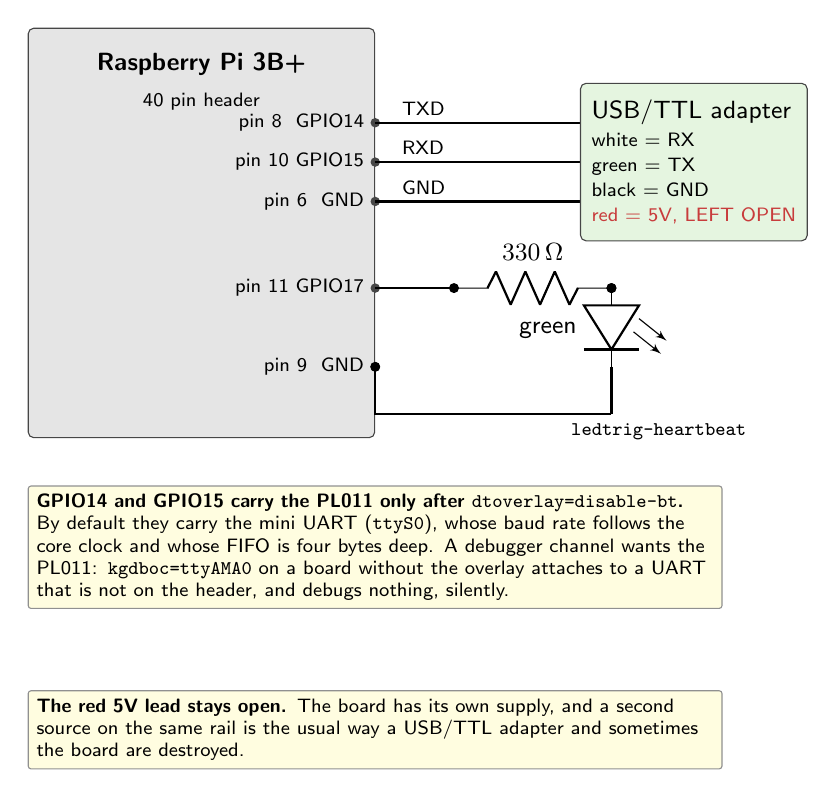
\begin{tikzpicture}[font=\sffamily\small]

  %% ---------------- the header ----------------
  \node[hw, minimum width=44mm, minimum height=52mm, align=center] (hdr) {};
  \node[font=\sffamily\small\bfseries, anchor=north] at ($(hdr.north)+(0,-2mm)$)
       {Raspberry Pi 3B+};
  \node[font=\sffamily\scriptsize, anchor=north] at ($(hdr.north)+(0,-7mm)$)
       {40 pin header};

  \coordinate (p8)  at ($(hdr.east)+(0,14mm)$);
  \coordinate (p10) at ($(hdr.east)+(0,9mm)$);
  \coordinate (p6)  at ($(hdr.east)+(0,4mm)$);
  \coordinate (p11) at ($(hdr.east)+(0,-7mm)$);
  \coordinate (p9)  at ($(hdr.east)+(0,-17mm)$);

  \foreach \p/\name in {p8/{pin 8\ \ GPIO14}, p10/{pin 10\ GPIO15},
                        p6/{pin 6\ \ GND}, p11/{pin 11\ GPIO17},
                        p9/{pin 9\ \ GND}} {
    \fill[linecol] (\p) circle (0.6mm);
    \node[font=\sffamily\scriptsize, anchor=east, inner sep=1pt]
         at ($(\p)+(-1mm,0)$) {\name};
  }

  %% ---------------- the console cable ----------------
  \draw[thick] (p8)  -- ++(26mm,0) coordinate (t8);
  \draw[thick] (p10) -- ++(26mm,0) coordinate (t10);
  \draw[thick] (p6)  -- ++(26mm,0) coordinate (t6);

  \node[font=\sffamily\scriptsize, anchor=south west, inner sep=1pt]
       at ($(p8)+(3mm,0.5mm)$)  {TXD};
  \node[font=\sffamily\scriptsize, anchor=south west, inner sep=1pt]
       at ($(p10)+(3mm,0.5mm)$) {RXD};
  \node[font=\sffamily\scriptsize, anchor=south west, inner sep=1pt]
       at ($(p6)+(3mm,0.5mm)$)  {GND};

  \node[host, right=0mm of t10, anchor=west, align=left, minimum height=20mm]
       (ttl) {USB/TTL adapter\\[-1pt]
              \scriptsize white = RX\\[-2pt]
              \scriptsize green = TX\\[-2pt]
              \scriptsize black = GND\\[-2pt]
              \scriptsize \textcolor{badcol}{red = 5V, LEFT OPEN}};

  %% ---------------- the heartbeat LED ----------------
  \draw[thick] (p11) -- ++(10mm,0) coordinate (r1);
  \draw (r1) to[R, l=\SI{330}{\ohm}, *-*] ++(20mm,0) coordinate (r2);
  \draw (r2) to[leD, l_=green, *-] ++(0,-10mm) coordinate (lk);
  \draw[thick] (lk) -- ($(lk)+(0,-6mm)$) coordinate (gnd);
  \draw[thick] (gnd) -| (p9);
  \node[circ] at (p9) {};

  \node[font=\sffamily\scriptsize, anchor=north, align=center]
       at ($(r2)+(6mm,-16mm)$) {\texttt{ledtrig-heartbeat}};

  %% ---------------- the two notes that matter ----------------
  \node[umlnote, anchor=north west, text width=86mm, align=left]
       at ($(hdr.south west)+(0,-6mm)$)
       {\textbf{GPIO14 and GPIO15 carry the PL011 only after}
        \texttt{dtoverlay=disable-bt}\textbf{.} By default they carry the
        mini UART (\texttt{ttyS0}), whose baud rate follows the core clock
        and whose FIFO is four bytes deep. A debugger channel wants the
        PL011: \texttt{kgdboc=ttyAMA0} on a board without the overlay
        attaches to a UART that is not on the header, and debugs nothing,
        silently.};

  \node[umlnote, anchor=north west, text width=86mm, align=left]
       at ($(hdr.south west)+(0,-32mm)$)
       {\textbf{The red 5V lead stays open.} The board has its own supply,
        and a second source on the same rail is the usual way a USB/TTL
        adapter and sometimes the board are destroyed.};

\end{tikzpicture}
\end{document}
